\section{Diseño de la Interfaz Gráfica de Usuario (GUI)}
\label{subsec:diseno_gui}

El desarrollo de la interfaz gráfica de usuario (GUI) parte de la premisa de que debe ser simple y contener lo mínimo necesario para los operadores que lo van a usar.

Para realizar un desarrollo ágil, intuitivo y desacoplado, se utilizó la herramienta de diseño \textbf{Qt Designer}, que permite un modelado visual mediante la técnica de arrastrar y soltar componentes gráficos.

Posteriormente, esta interfaz visual se compiló mediante la biblioteca \textbf{PySide6} para su integración con el resto del programa, asegurando la compatibilidad con el lenguaje \textbf{Python} bajo el patrón de arquitectura MVP.

El diseño de la GUI se estructuró a partir de los requerimientos y la retroalimentación directa con los técnicos de laboratorio encargados del ensayo de impulso atmosférico tipo rayo.

\textbf{Requisitos de la GUI:}
\begin{itemize}
    \item Registrar datos del elemento bajo ensayo.
    \item Registrar de condiciones ambientales (temperatura, humedad y presión).
    \item Control centralizado del osciloscopio digital (ajuste de escalas, bases de tiempo, posición del cursor y modos de disparo).
    \item Almacenar la información manualmente.
    \item Exportar resultados a hojas de cálculo.
\end{itemize}

En base a esos requisitos se desarrolló la interfaz, la cual puede observarse en las figuras \ref{fig:GUI_1366x768} y \ref{fig:GUI_1920x1080}, que tiene la capacidad de autoajustar sus dimensiones al tamaño de la pantalla, siendo particularmente diseñado para las dos configuraciones más comunes al momento de este desarrollo, que son $1366 \times 768$ px y $1920 \times 1080$ px.

\begin{figure}[H]
    \centering
    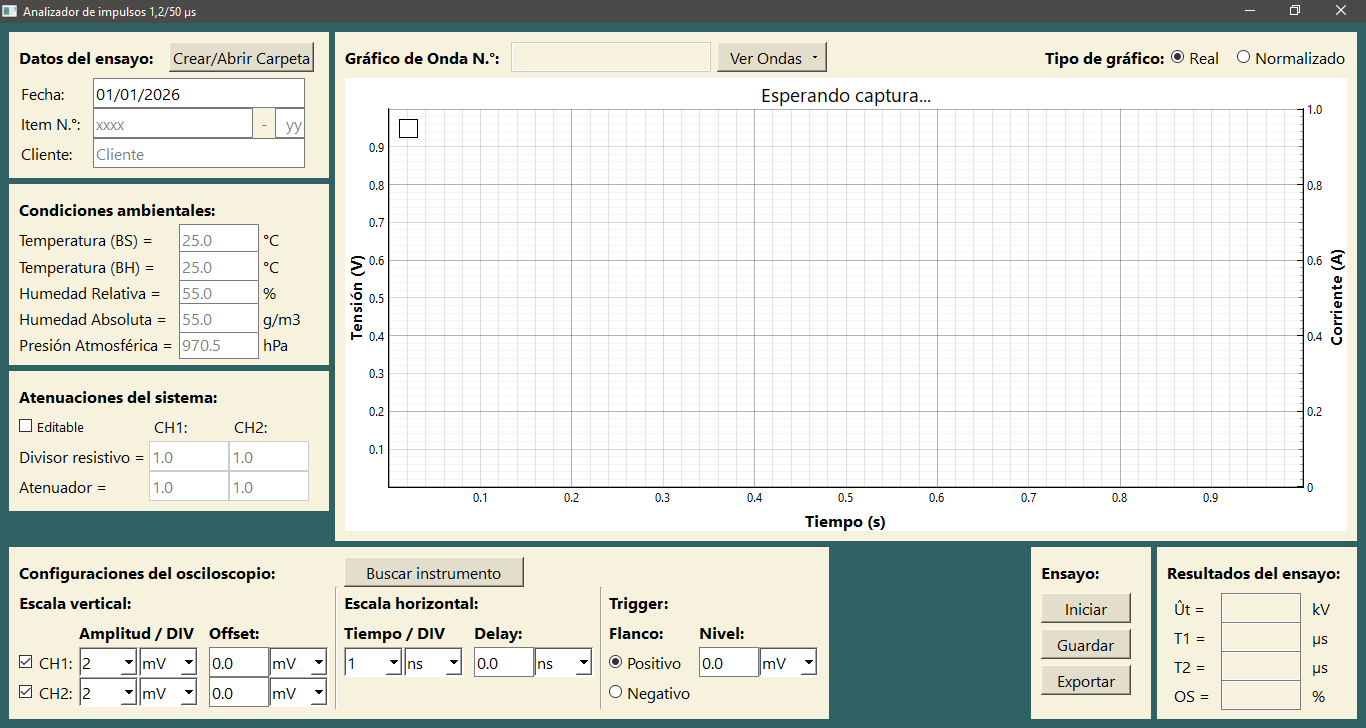
\includegraphics[width=1\textwidth]{img/GUI_1366x768.png}
    \caption{GUI en tamaño 1366x768 px.}
    \label{fig:GUI_1366x768}
\end{figure}

\begin{figure}[H]
    \centering
    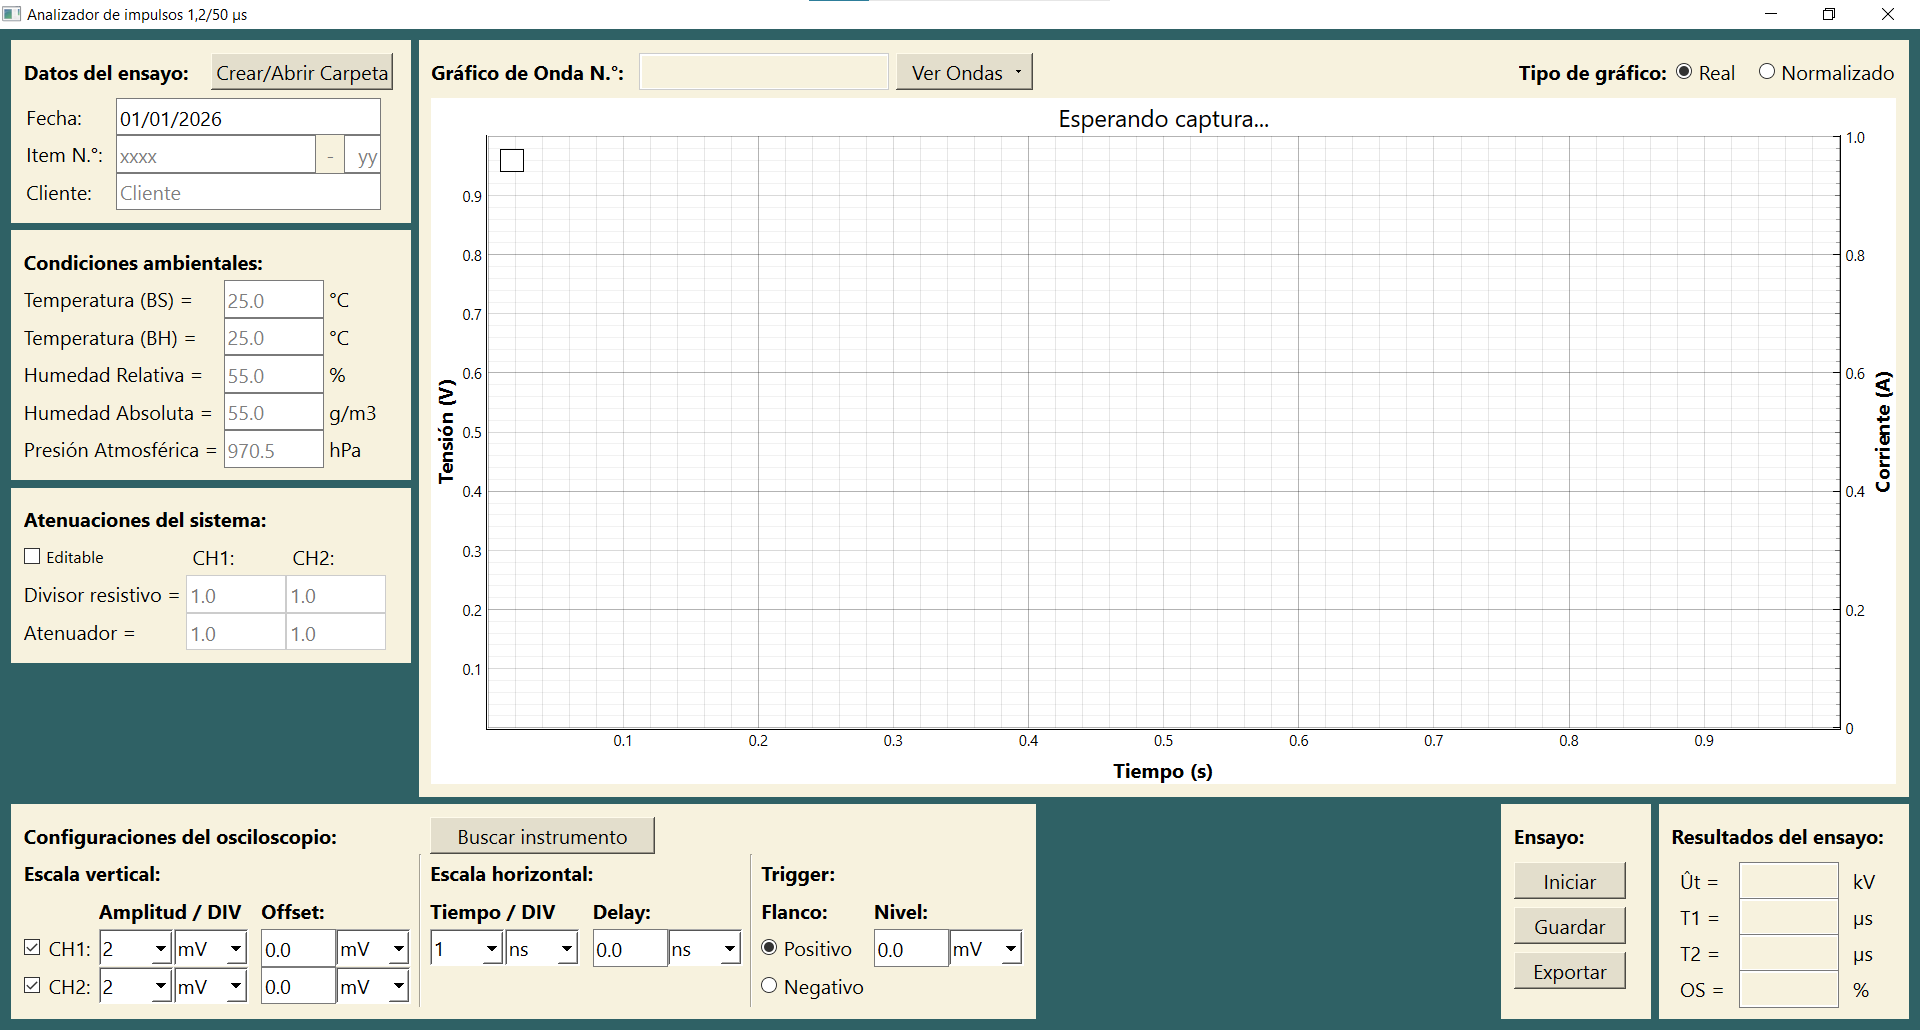
\includegraphics[width=1\textwidth]{img/GUI_1920x1080.png}
    \caption{GUI en tamaño 1920x1080 px.}
    \label{fig:GUI_1920x1080}
\end{figure}

Con el fin de que sea intuitivo para los operadores, se trazo un recorrido lógico para trabajar en la ventana.

\begin{figure}[H]
    \centering
    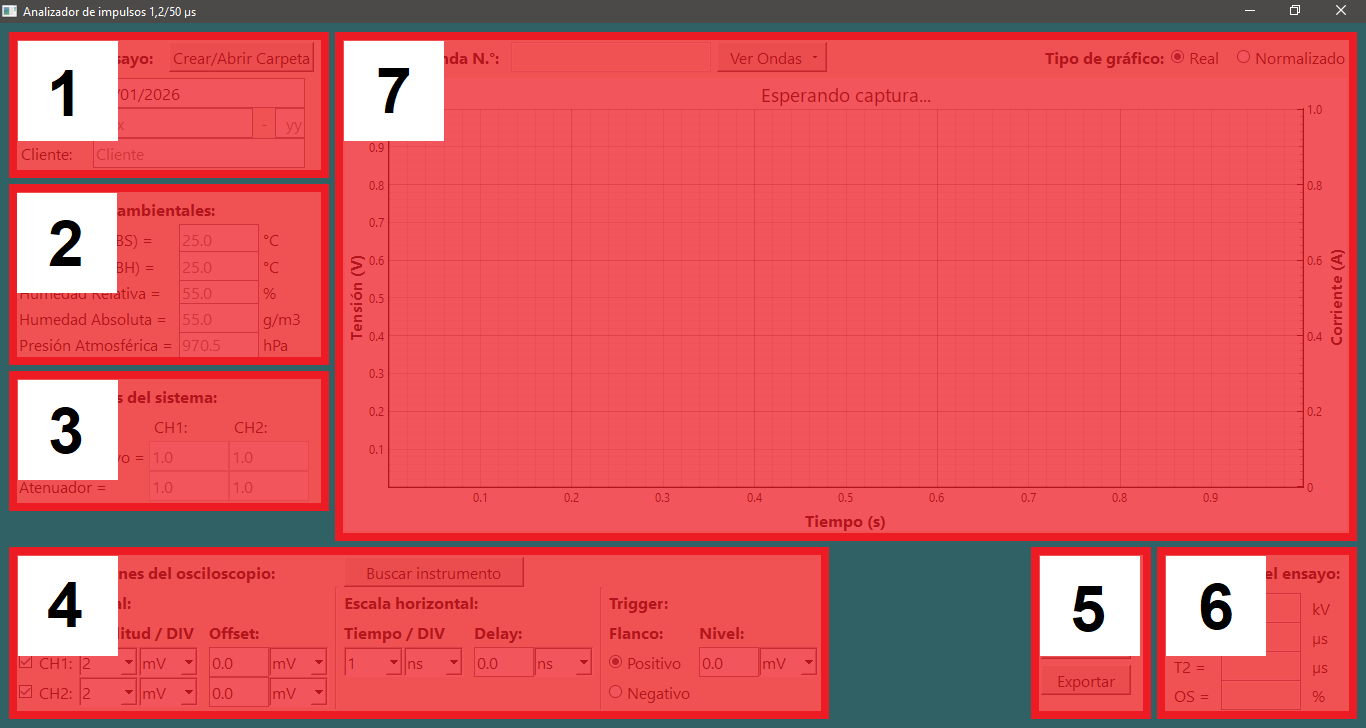
\includegraphics[width=1\textwidth]{img/GUI - bloques.png}
    \caption{Recorrido de trabajo.}
    \label{fig:recorrido_gui}
\end{figure}


\begin{enumerate}
    \item \textbf{Datos del ensayo}: Sirve para cargar los datos relacionados a la trazabilidad del laboratorio sobre del elemento que se va a ensayar.
    \item \textbf{Condiciones ambientales}: Donde el operador introduce parámetros termodinámicos de referencia como la temperatura, presión y humedad. Estos valores son esenciales para la posterior corrección atmosférica de la tensión de ensayo $U_t$ de acuerdo con la norma \textbf{IEC 60060-1} \cite{iec60060_1}
    \item \textbf{Atenuaciones del sistema}: Para ingresar los factores de atenuación de los divisores resistivos y atenuadores coaxiales, correspondientes al sistema de medición.
    \item \textbf{Configuraciones del osciloscopio}: Agrupa los comandos de control del instrumento
    \item \textbf{Ensayo}: Permite al usuario ejecutar la adquisición de señal, guardar los registros en la base de datos y realizar la exportación en formatos planos como Excel o CSV.
    \item \textbf{Resultados del ensayo}: Este panel renderiza dinámicamente en una tabla los parámetros de la onda calculados tras la adquisición ($U_t$, $T_1$, $T_2$ o $T_c$ y $OS\%$).
    \item \textbf{Gráfico de ondas}: El área de mayor tamaño de la pantalla se reservó para el renderizado de las curvas de tensión y corriente.
\end{enumerate}
